\section{Pruebas}
Uno de los pilares de \ac{xp} es el proceso de pruebas. Esta metodolog�a de desarrollo anima a probar constantemente tanto como sea posible. Esto permite aumentar la calidad de los sistemas reduciendo el n�mero de errores no detectados y disminuyendo el tiempo transcurrido entre la aparici�n de un error y su detecci�n. Tambi�n permite aumentar la seguridad de evitar efectos colaterales no deseados a la hora de realizar  dise�ada por los programadores, y pruebas de aceptaci�n o pruebas funcionales destinadas a evaluar si al final de una iteraci�n se consigui� la funcionalidad requerida dise�adas por el cliente final \citep{gutierrez2006pruebas}.
Con el objetivo de comprobar que las funcionalidades implementadas funcionan de acuerdo a las especificaciones descritas por el cliente, se realizaron pruebas unitarias. %TODO y pruebas de sitema

\subsection{Pruebas unitarias}
\label{ss:unit-tests}
Las pruebas unitarias son una forma de comprobar que un fragmento de c�digo funciona correctamente.Son peque�os tests que validan el comportamiento de un objeto y la l�gica \citep{gutierrez2006pruebas}. \ac{xp} plantea la realizaci�n de pruebas unitarias continuas, frecuentemente repetidas y automatizadas, incluyendo pruebas de regresi�n, y aconseja escribir el c�digo de la prueba antes de la codificaci�n \citep{kniberg2007scrumyxp}.\\
Para la aplicaci�n de las pruebas unitarias a la soluci�n se emple� el framework JUnit el cual permite realizar la ejecuci�n de clases Java de manera controlada, para poder evaluar si el funcionamiento de cada uno de los m�todos de la clase se comporta como se espera. Es decir, en funci�n de alg�n valor de entrada se eval�a el valor de retorno esperado; si la clase cumple con la especificaci�n, entonces JUnit devolver� que el m�todo de la clase pas� exitosamente la prueba; en caso de que el valor esperado sea diferente al que regres� el m�todo durante la ejecuci�n, JUnit devolver� un fallo en el m�todo correspondiente.
\begin{figure}[htp]
	\centering
	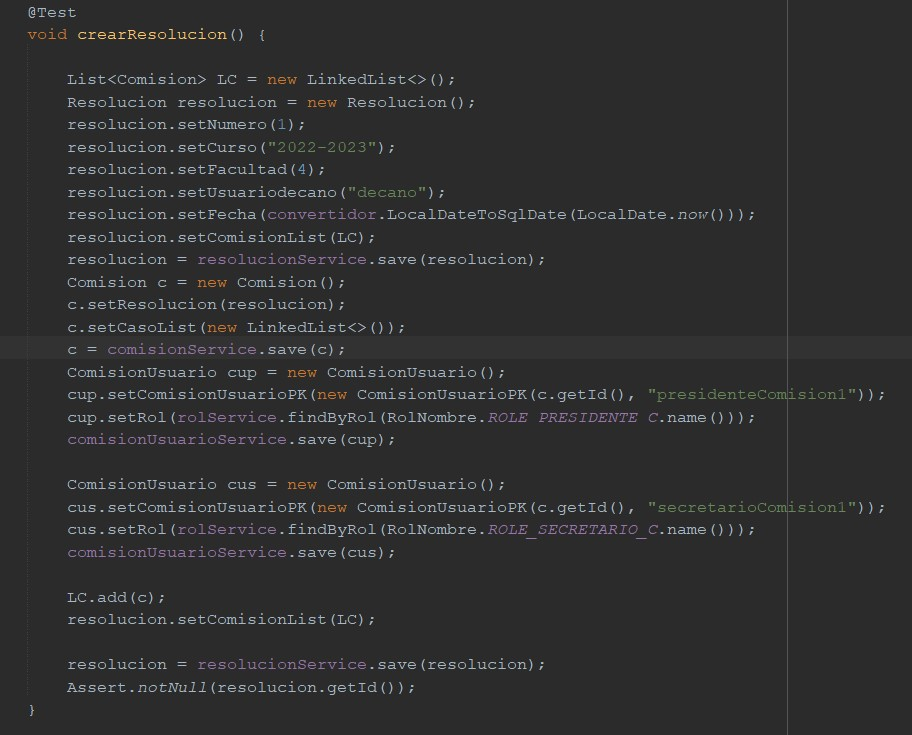
\includegraphics[width=0.8\textwidth]{images/test/PU1.jpg}
	\caption{Resultado de la ejecuci�n de pruebas unitarias en el c�digo fuente de CDIS. parte 1.}
	\label{fig:pu1}
\end{figure}
\begin{figure}[htp]
	\centering
	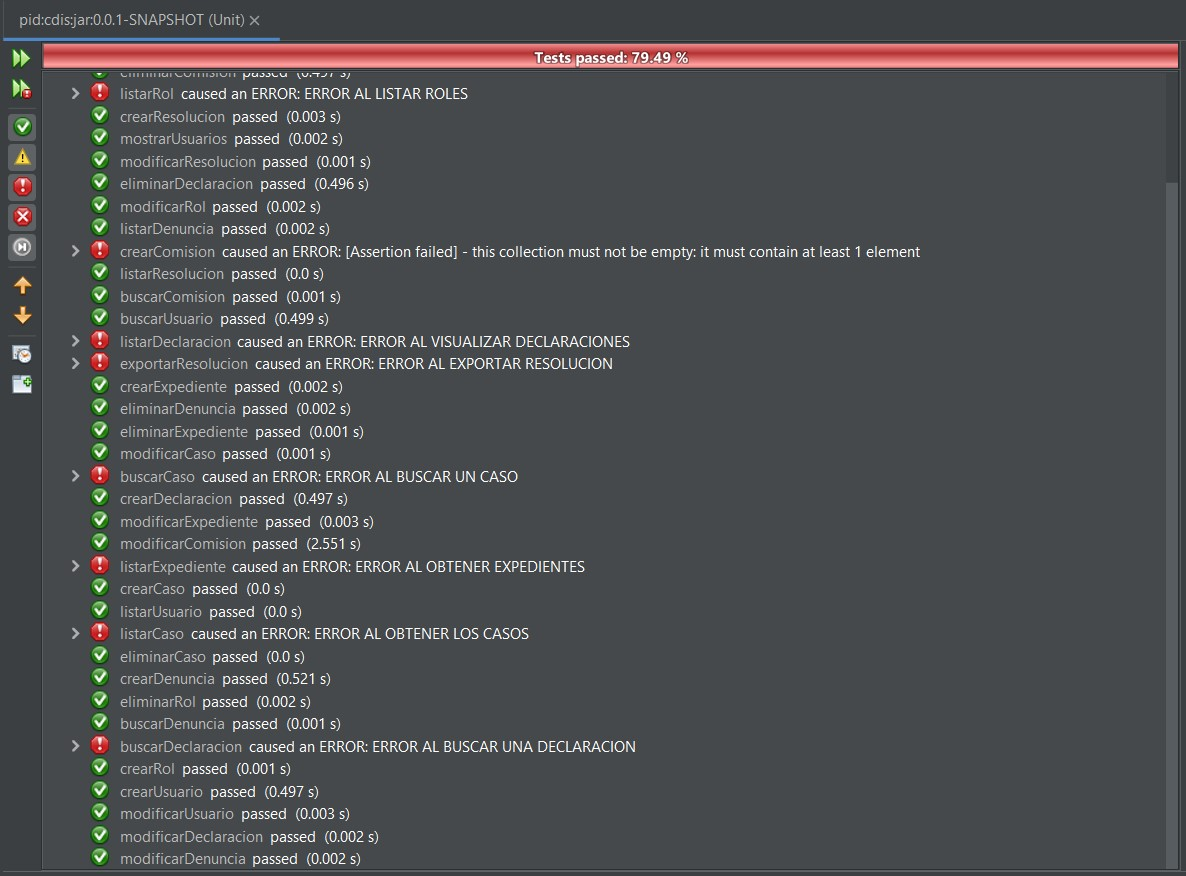
\includegraphics[width=0.8\textwidth]{images/test/PU2.jpg}
	\caption{Resultado de la ejecuci�n de pruebas unitarias en el c�digo fuente de CDIS. parte 2.}
\end{figure}

Se realizaron 39 pruebas unitarias al c�digo de las cuales 1 fue
fallida y se corrigi� exitosamente. A continuaci�n, se muestra el c�digo antes
de corregir el error detectado en la figura \ref{fig:pu1}:

\begin{figure}[htp]
	\centering
	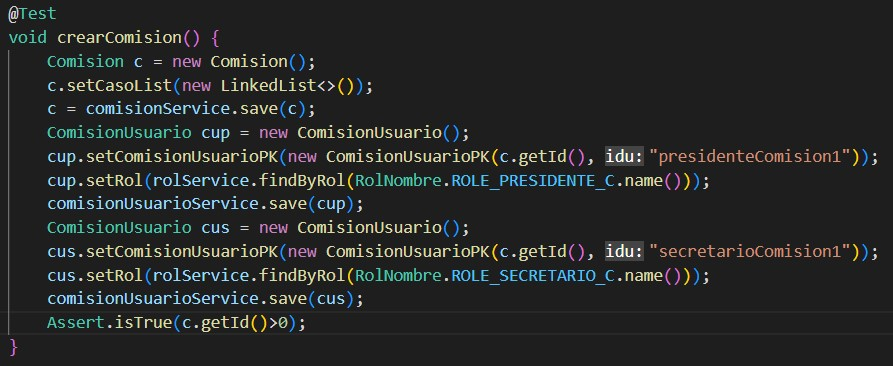
\includegraphics[width=0.8\textwidth]{images/test/before-error.jpg}
	\caption{M�todo crearComisi�n con error}
\end{figure}

Como se puede apreciar se est� intentando crear una comisi�n, pero por
alg�n motivo la l�gica del c�digo no fue bien planteada y terminamos
recibiendo una excepci�n causada a ra�z de que para crear una comisi�n
disciplinaria hace falta tambi�n asignarle una resoluci�n que la
contenga. La soluci�n a dicho problema se encuentra en la imagen
siguiente:
\clearpage
\begin{figure}[htp]
	\centering
	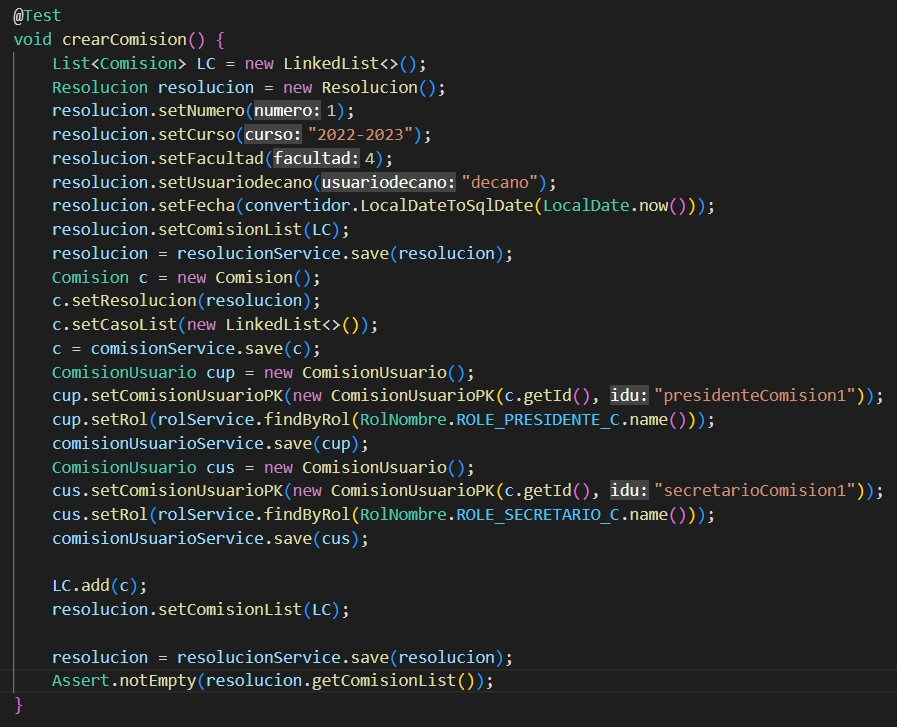
\includegraphics[width=0.8\textwidth]{images/test/after-error.jpg}
	\caption{M�todo crearComisi�n corregido}
\end{figure}

De esta forma garantizamos que una resoluci�n contiene la comisi�n que
estamos creando y esta se puede guardar con normalidad en la base de
datos.

Ahora se mostrar�n algunas im�genes de otras pruebas exitosas:

\begin{figure}[htp]
	\centering
	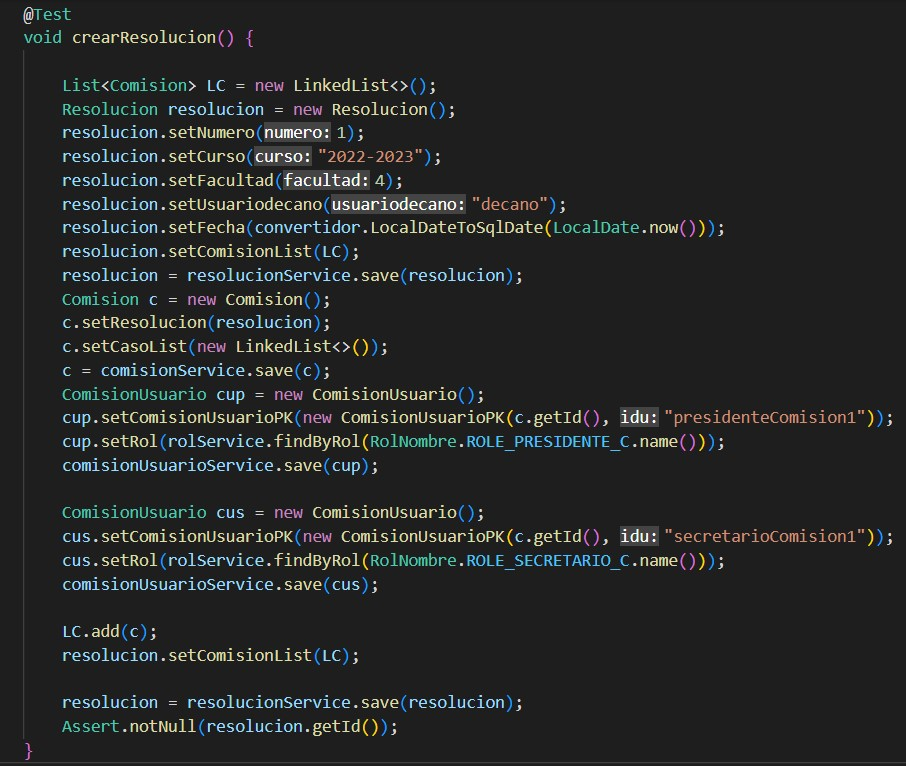
\includegraphics[width=0.8\textwidth]{images/test/E1.jpg}
	\caption{prueba para crearResoluci�n()}
\end{figure}

Se hace una prueba para crearResoluci�n(): Se comprueba que la
creaci�n de una resoluci�n sea exitosa despu�s de asignarle una comisi�n
disciplinaria

\begin{figure}[htp]
	\centering
	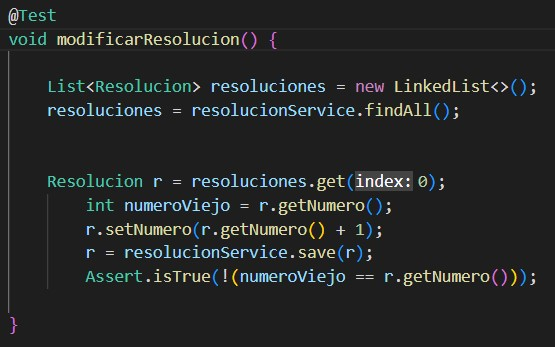
\includegraphics[width=0.8\textwidth]{images/test/E2.jpg}
	\caption{prueba para modificarResolucion()}
\end{figure}

Se hace una prueba para modificarResolucion(): Se actualiza la
informaci�n de una resoluci�n ya creada buscando fallas

\begin{figure}[htp]
	\centering
	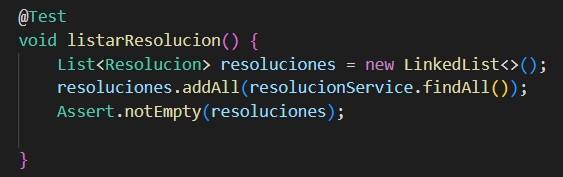
\includegraphics[width=0.8\textwidth]{images/test/E3.jpg}
	\caption{prueba para listarResolucion()}
\end{figure}

Se hace una prueba para listarResolucion(): Se llaman objetos
de la base de datos para guardarlos en un listado de objetos
de tipo: Resolucion

\begin{figure}[htp]
	\centering
	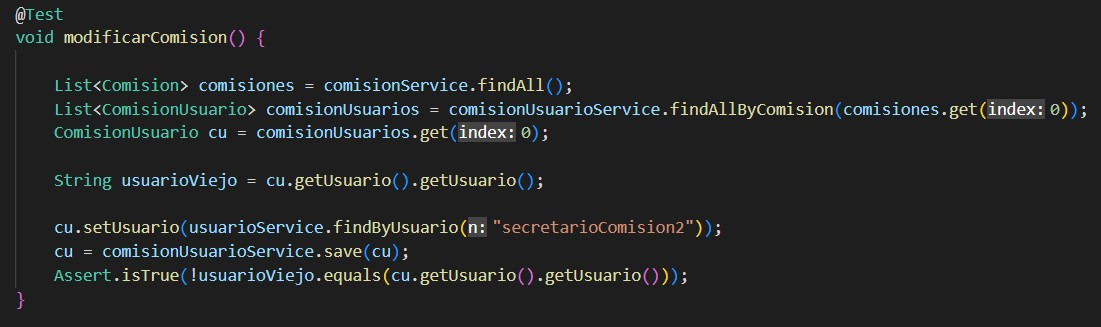
\includegraphics[width=0.8\textwidth]{images/test/E4.jpg}
	\caption{prueba para modificarComision()}
\end{figure}

Se hace una prueba para modificarComision(): Se actualiza la
informaci�n de una comisi�n seleccionada buscando fallas

\begin{figure}[htp]
	\centering
	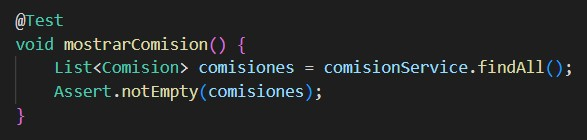
\includegraphics[width=0.8\textwidth]{images/test/E5.jpg}
	\caption{prueba para mostrarComisionl()}
\end{figure}

Se hace una prueba para mostrarComisionl(): Se llama a la
base de datos para obtener objetos de tipo: Comision

\begin{figure}[htp]
	\centering
	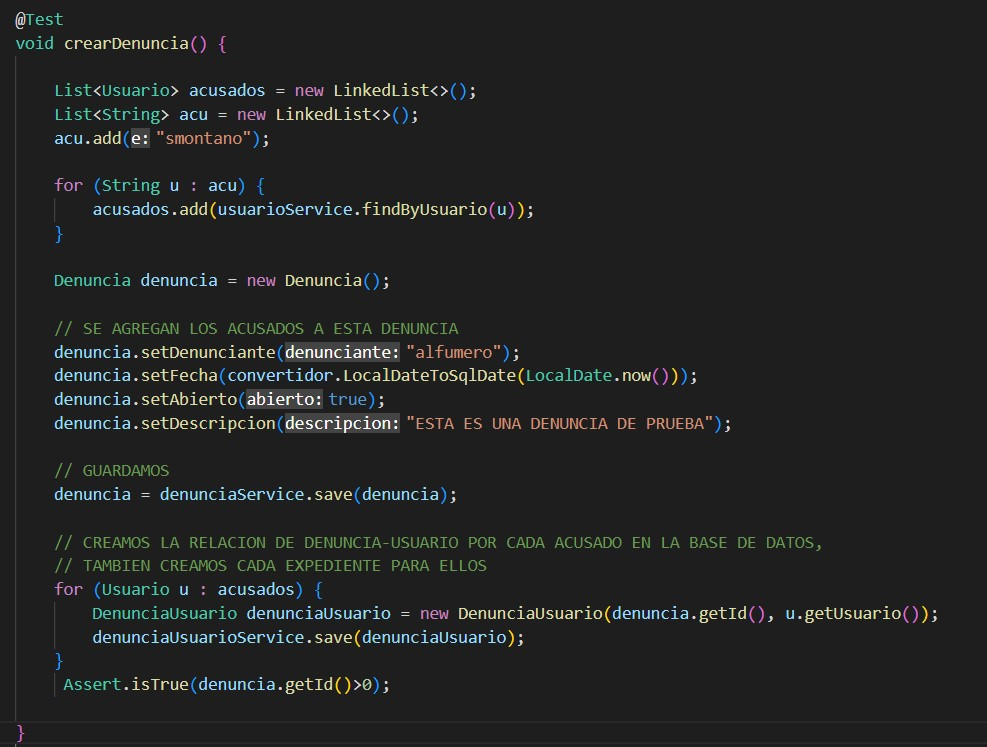
\includegraphics[width=0.8\textwidth]{images/test/E6.jpg}
	\caption{prueba para crearDenuncia()}
\end{figure}

Se hace una prueba para crearDenuncia(): Se crea una denuncia,
este es uno de los m�todos m�s importantes y base de la aplicaci�n

\begin{figure}[htp]
	\centering
	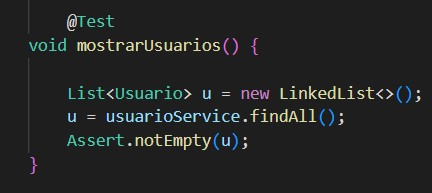
\includegraphics[width=0.8\textwidth]{images/test/E7.jpg}
	\caption{prueba para mostrarUsuarios()}
\end{figure}

Se hace una prueba para mostrarUsuarios(): Se comprueba que todos
los usuarios se muestren correctamente

\begin{figure}[htp]
	\centering
	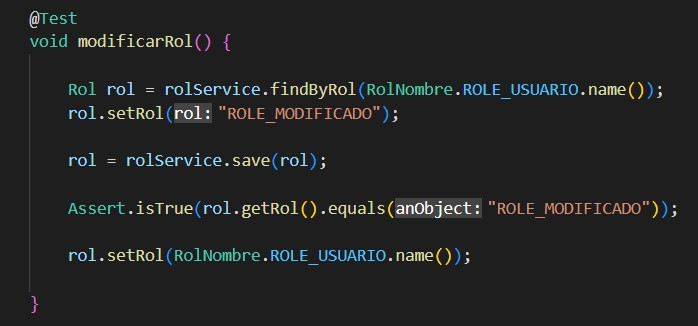
\includegraphics[width=0.8\textwidth]{images/test/E8.jpg}
	\caption{prueba para modificarRol()}
\end{figure}

se hace un test para modificarRol(): Se comprueba el correcto
funcionamiento en la actualizaci�n de los atributos del objeto de prueba de tipo: Rol

\clearpage

%\subsection{Pruebas de aceptaci�n}
Las pruebas de aceptaci�n son definidas por el usuario del sistema y preparadas por el equipo de desarrollo, aunque la ejecuci�n y aprobaci�n final corresponden al usuario. Estas pruebas van dirigidas a comprobar que el sistema cumple los requisitos de funcionamiento esperado, recogidos en el cat�logo de requisitos y en los criterios de aceptaci�n del sistema de informaci�n, y conseguir as�? la aceptaci�n final del sistema por parte del usuario \citep{gutierrez2006pruebas}.
A continuaci�n se muestran algunas de las pruebas de aceptaci�n realizadas. 

\begin{acceptancetest}[t:hu1p1] % label in brackets
   \testcasecode{HU1\_P1}
   \testcasedescription{Prueba para la funcionalidad: Autenticar usuario. Prueba que s�lo se puede acceder a las funcionalidades del sistema si se ha realizado una autenticaci�n exitosa primero}
   \testcaseexeccond{El usuario no est� autenticado en el sistema.}
   \testcaseexecstep{
   \begin{enumerate}
   \item Se navega a la p�gina donde se encuentra el formulario de autenticaci�n.
   \item Se ingresan los credenciales correctos en el formulario de autenticaci�n.
   \item Se inicia la autenticaci�n a trav�z del bot�n de acci�n del formulario o la tecla Enter.
   \item Se recarga la p�gina.
   \end{enumerate}
   }
   \testcaseexpresult{El usuario queda autenticado en el sistema si se ingresan los credenciales correctos solamente. Se muestran los elementos de la interfaz que permiten acceder a las funcionalidades del sistema y la informaci�n del usuario autenticado justo despu�s de culminar el proceso de autenticaci�n.\\
      Evaluaci�n de la prueba: Satisfactoria}
   \testcasename{Autenticar usuario}
   \testcaseuserstory{1}
\end{acceptancetest}

\begin{acceptancetest}[t:hu1p2] % label in brackets
   \testcasecode{HU1\_P2}
   \testcasedescription{Prueba para la funcionalidad: Autenticar usuario. Prueba que el usuario puede cerrar una sesi�n iniciada.}
   \testcaseexeccond{El usuario est� autenticado en el sistema.}
   \testcaseexecstep{
   \begin{enumerate}
   \item Se inicia el cierre de sesi�n desde el men� del cliente.
   \item Se confirma la acci�n en un cuadro de di�logo.
   \item Se recarga la p�gina.
   \end{enumerate}
   }
   \testcaseexpresult{El usuario deja de estar autenticado en el sistema.\\
   Evaluaci�n de la prueba: Satisfactoria}
   \testcasename{Autenticar usuario}
   \testcaseuserstory{1}
\end{acceptancetest}